% !Mode::"TeX:UTF-8"
\documentclass[a4paper, 12pt]{ctexart}

\newcommand{\LstlistingLabel}[1]{代码#1}
\newcommand{\EquationLabel}[1]{式(#1)}
\newcommand{\FigureLabel}[1]{图#1}
\newcommand{\TableLabel}[1]{表#1}
\newcommand{\ProblemLabel}[1]{问题#1}

\newcommand{\ProblemLang}{问题}
\newcommand{\NoteLang}{注}
\newcommand{\ProofLang}{证明}
\newcommand{\SolutionLang}{解}
\newcommand{\LstlistingLang}{代码}

\usepackage{enumerate}
\usepackage{float} % [H].
\usepackage{fontspec} % fonts.
\usepackage{subcaption} % subcaption and subfigure.
\usepackage[dvipsnames]{xcolor} % 颜色声明.

\usepackage{geometry}
\geometry{left=2.5cm, right=2.5cm, top=2.5cm, bottom=2.5cm}

\usepackage{amsmath}
\usepackage{amssymb}
\usepackage{commath} % abs, norm

\usepackage[math-style=TeX, bold-style=TeX, partial=upright]{unicode-math}
\setmathfont{XITS Math}
\setmathfont[range={\mathcal,\mathbfcal}, StylisticSet=1]{XITS Math} % Script

\newcommand*{\diff}{\mathop{}\!\symup{d}}
\newcommand*{\matr}[1]{\symsfit{#1}}
\newcommand*{\vect}[1]{\symbf{#1}}

\usepackage{pgfplotstable} % Need to load before xwatermark
\usepackage{booktabs}

\pgfplotsset{width=7cm, compat=1.16}

\pgfplotstableset{
    every head row/.style={before row=\toprule, after row=\midrule},
    every last row/.style={after row=\bottomrule}
}

\usepackage{caption}

\captionsetup{
    margin    =   6pt,
    font      =   small,
    labelfont =   bf
}

\usepackage{fancyhdr}

\usepackage{graphicx}

\graphicspath{{resources/}}

\usepackage{hyperref}

\hypersetup{
    linktoc             =   all,
    colorlinks          =   true,
    linkcolor           =   cyan,
    anchorcolor         =   black,
    citecolor           =   green,
    filecolor           =   cyan,
    menucolor           =   red,
    runcolor            =   filecolor,
    urlcolor            =   magenta,
    bookmarksnumbered   =   true,
    pdfstartview        =   FitH,
    pdfpagelayout       =   OneColumn
}

\usepackage{listings}
\usepackage{letltxmacro} % \let
\usepackage[numbered, framed]{matlab-prettifier}
\usepackage[T1]{fontenc}

%% Title

\renewcommand\lstlistingname{\LstlistingLang}
% \renewcommand\lstlistlistingname{代码} % We don't use the list of listings

\lstset{
    breaklines=true,
    backgroundcolor=\color{lightgray},
    basicstyle=\scriptsize,
    inputpath=resources/,
    numbers=left,
    numberstyle={\color{black!33}\scriptsize\sffamily},
    xleftmargin=2em,
    xrightmargin=2em
}

%% Lstinline with color box

\LetLtxMacro{\oldlstinline}{\lstinline}
\renewcommand{\lstinline}[2][]{\colorbox{lightgray}{\oldlstinline[#1]{#2}}}

%% MATLAB presets

\newcommand{\matlabinline}[1]{
    \lstinline[style=MATLAB-editor, basicstyle=\mlttfamily]{#1}
}
\newcommand{\matlabinputlisting}[2][]{ % #1: caption or label
    \lstinputlisting[
        style=MATLAB-editor,
        basicstyle=\mlttfamily\scriptsize,
        #1
    ]{#2}
}

\usepackage{varioref} % For Cross References.

\labelformat{lstlisting}{\LstlistingLabel{#1}}
\labelformat{equation}{\EquationLabel{#1}}
\labelformat{figure}{\FigureLabel{#1}}
\labelformat{table}{\TableLabel{#1}}
\labelformat{problem}{\ProblemLabel{#1}}

\usepackage{pgfplots}
\pgfplotsset{width=7cm, compat=1.15}
\usepgfplotslibrary{external}
\tikzsetexternalprefix{tikz/}
\tikzexternalize

\title{基于EM算法的ATM交易状态特征分析与异常检测}
\date{\today}
\author{}

\begin{document}
    \pagestyle{plain}
    \maketitle
    \begin{table}[H]
        \begin{center}
            \pgfplotstabletypeset[
                columns/a/.style={column name=工作量, string type},
                columns/b/.style={column name=姓名, string type},
                columns/c/.style={column name=学号, string type},
                columns/d/.style={column name=具体工作, string type},
            ]{
                a b c d
                1/3 张赫(队长) 1752114 {统筹安排, 问题三和摘要}
                1/3 李瑞 1752516 {文章整体思路和交易量部分}
                1/3 陈旭阳 1753763 {论文排版, 成功率和响应时间部分}
            }
        \end{center}
    \end{table}
    \clearpage

    % !TeX root = ../main.tex

% 中英文摘要和关键字

\begin{abstract}{代数几何, 交换代数, 准素分解, 维数理论}
  这篇文章主要面向没有接触过但想要了解代数几何的本科生, 旨在以尽可能少的前置知识向读者自洽地展示代数几何的基础.

  代数几何的理论根基在于代数. 本文从基本定义开始建立了以环论为主模论为辅的交换代数理论, 研究了商环与分式环的基本性质, 证明了Noether环上准素分解的存在性及其满足的唯一性, 以域论为基础利用Noether正规化引理证明了域的有限生成整环上的维数定理和Hilbert零点定理.

  代数几何的研究对象在于几何. 本文研究了固定代数闭域上的仿射与射影空间中的代数集, 建立了根式理想与代数集之间的对应, 一次将准素分解理论与几何相联系. 本文还讨论了代数簇上的函数结构, 以此将维数理论应用到几何中, 并证明了两组代数范畴与几何范畴的等价. 最后本文简要介绍了概形的概念, 其相比于代数簇能更完整地体现代数所提供的信息. 读完本文, 读者可以初步掌握代数几何基础, 并做好进一步学习重要技术的准备.
\end{abstract}

\begin{abstract*}{algebraic geometry, commutative algebra, primary decomposition, dimension theory}
  \lipsum[1-2]
\end{abstract*}

    \clearpage

    \section{模型假设}

    \begin{enumerate}
    \item 交易状态异常会造成交易数目, 交易成功率, 交易响应时间数据至少其一产生异常.\\
    \item 提供的观测数据是真实准确的.\\
    \item 每次交易是否成功是独立同分布的随机事件. 特别的, 各种故障是否发生是独立同分布的随机事件.\\
    \item 除系统自身运行中产生的故障或异常外, 所有会对ATM机交易数目, 交易成功率, 交易响应时间数据造成影响的客观性质完全相同.\\
\end{enumerate}


    \section{交易量特征参数与异常检测}

    \subsection{分析}

将1月23日至4月23日所有天的业务量时间序列按月汇总作图. 从图中可以看出个别天的数据很异常, 查日历知道2017年1月27日是除夕夜, 从实际因素分析, 本文推断可能是除夕前人们需要准备送礼或准备压岁钱ATM机导致交易量增加, 春节期间人们走亲访友导致交易量减少, 因此决定分段处理日总交易. 而不同日期的业务量峰值变化很大, 尤其是1月27日前业务量的峰值明显高于其他日期的业务量峰值. 1月27日后几天, 业务量峰值又明显小于其他日期. 除夕当天业务量从上午到下午有一个缓慢降低的过程. 这一点可从春节前人们大量购买年货, 春节后进入假期, 人们很少购物来解释.

\begin{figure}[H]
    \centering
    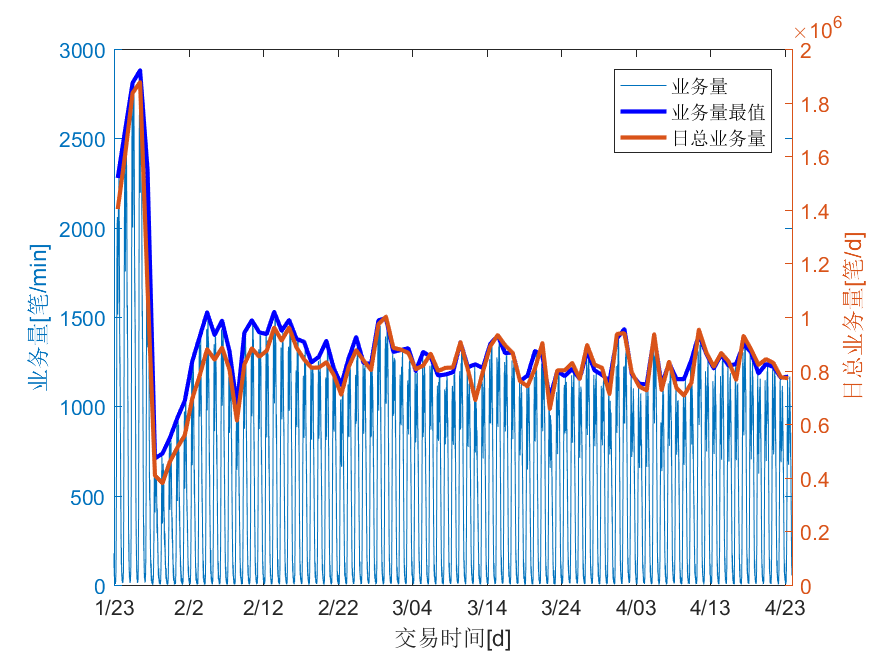
\includegraphics[width=7cm]{lr1.png}
    \caption{交易量随日期的变化}
\end{figure}

而在春节之后, 本文发现每日交易总量并没有明显的以七天为周期的变化规律. 因而难以发现其中工作日和休息日的交易变化区别. 为了简化问题, 所以本文假定工作日和非工作日的交易量不存在明显差别.

另外, 从上图中可以看出: 在1月23日至1月27日, 1月28日至2月1日的日平均交易量存在明显差别. 为了更加明显表示其区别, 本文在一张图上表示出这三段时间的平均交易量随时间的变化.

\begin{figure}[H]
    \centering
    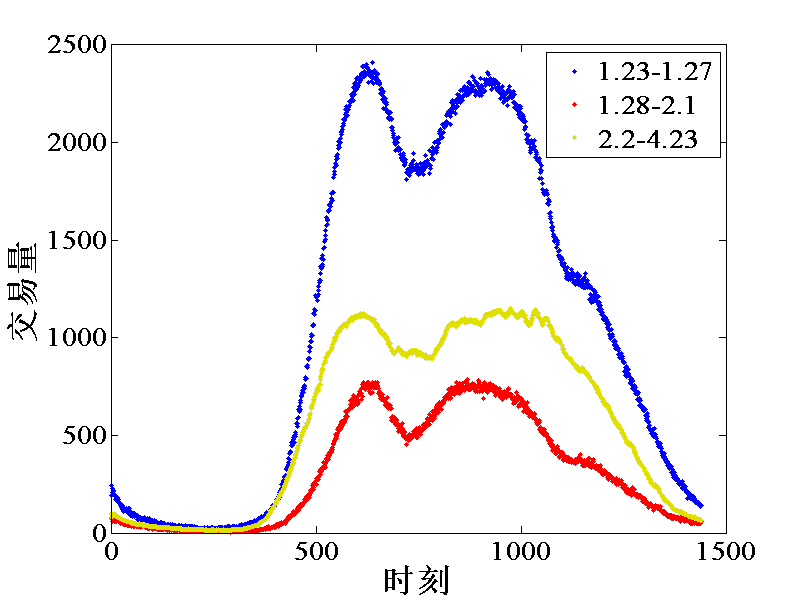
\includegraphics[width=7cm]{lr2.png}
    \caption{三段时间内平均交易量在一天各时刻的变化}
\end{figure}

由每日交易量随时间的变化图可知, 交易量在早晚各有一个高峰. 交易量的主要特征体现在早晚两个高峰中, 对交易量分布的分析也需要从这早晚两个高峰入手. 考虑到现实意义和模型的可操作性, 本文认为交易量在早晚高峰期分别满足满足两种不同的正态分布, 而总的交易分布, 应是这两个正态分布的合分布. 对于这种多参多峰的复杂分布, 在求解参数时, 为了使拟合分布与实际数据有着很好的贴合度, 本文打算利用EM算法来求双峰高斯函数的参数.

\subsection{特征参数选取}

EM算法分为两步: E(expectation)步, 求隐变量的期望.M(maximum)步, 求似然函数的最大值. 具体应用到多元高斯模型中, M步需要求解
\begin{figure}[H]
    \centering
    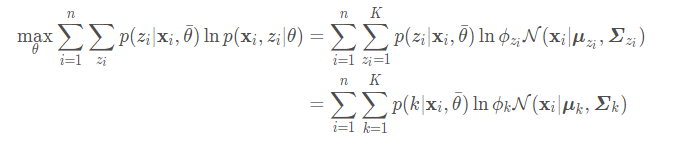
\includegraphics[width=14cm]{lr3.png}
\end{figure}

注意到$p(k|\vect{x}_{i}, \bar{\theta})$不包含优化变量$\theta$, 因此在此问题中可以看作关于$i$和$k$的常数, 故我们暂记其为$\gamma_{ik}$, 留到最后再讨论其具体取值. 忽略掉优化无关常数, M步的优化问题正式写作:
\begin{figure}[H]
    \centering
    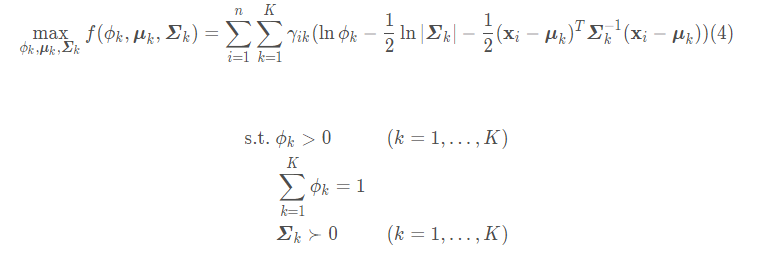
\includegraphics[width=14cm]{lr4.png}
\end{figure}

综上所述, 可得整个算法如下:
\begin{figure}[H]
    \centering
    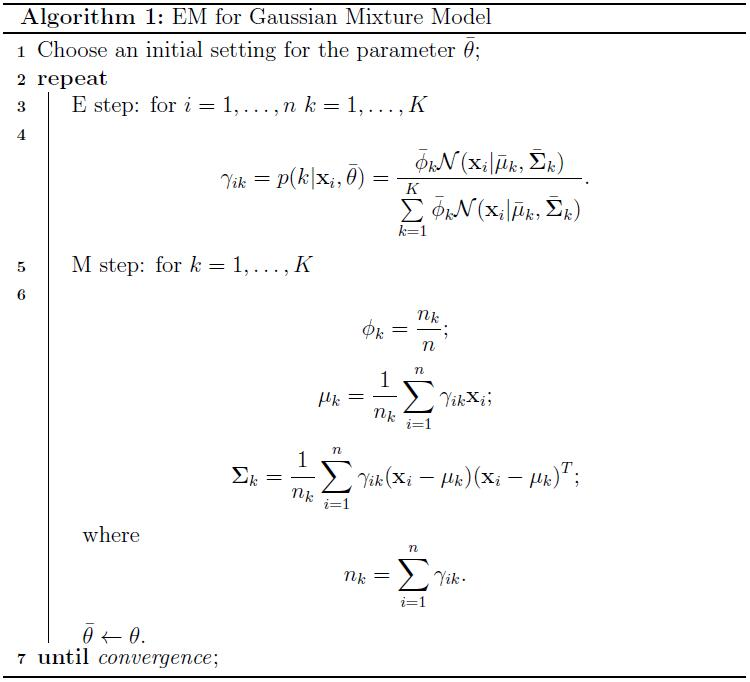
\includegraphics[width=14cm]{lr5.png}
\end{figure}

进行拟合求解后, 本文得到如下结果(以1月25日为例):

\begin{figure}[H]
    \begin{minipage}[b]{0.49\textwidth}
        \centering
        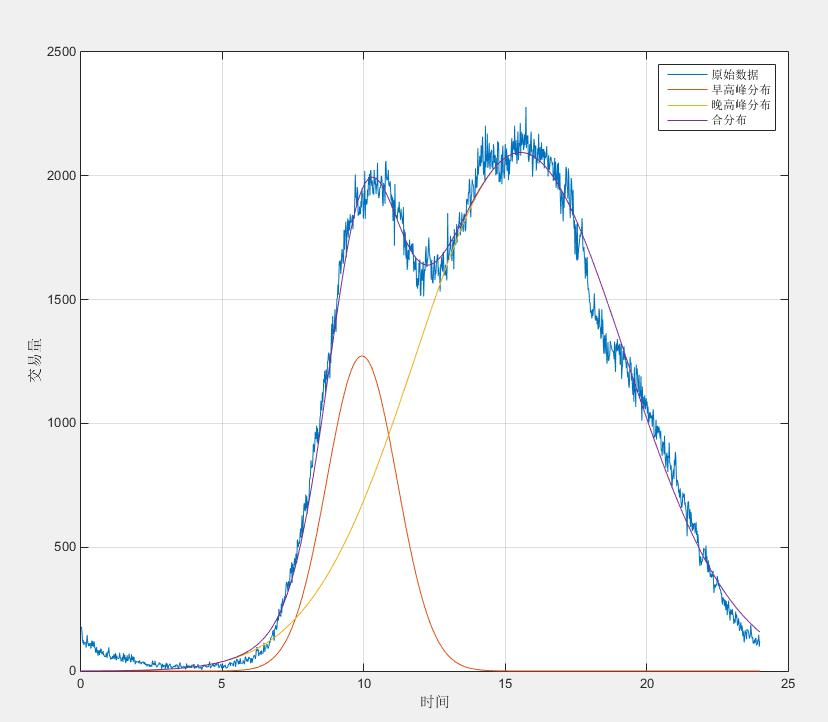
\includegraphics[width=7cm]{lr6.png}
        \captionof{figure}{1月25日交易量随时间分布拟合图像}
    \end{minipage}
    \hfill
    \begin{minipage}[b]{0.49\textwidth}
        \centering
        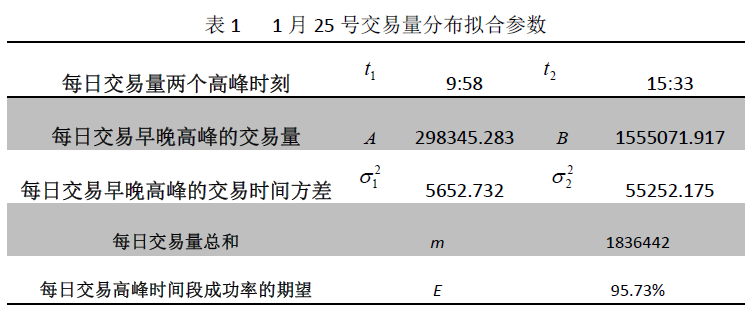
\includegraphics[width=7cm]{lr7.png}
        \captionof{figure}{1月25日交易量随时间分布拟合参数}
    \end{minipage}
\end{figure}


    \section{成功率特征参数与异常检测}

    \subsection{特征参数选取}

首先本文作出了成功率随交易量变化的散点图, 发现成功率在小交易量处波动较大, 在大交易量处很稳定, 其取值大约在96\%附近. 从直观上来说因系统出现异常或故障的次数与交易量之间呈正相关关系, 然而成功率这一参数并不满足这一要求, 因此只利用成功率的大小来衡量是否出现异常或故障是不足够的, 需要对其加以改进.

由模型假设, 每次交易是否成功为独立同分布的随机变量$X_{i}$, 设其均值为$\mu$, 方差为$\sigma^{2}$. 
设$R(m)$为$m$时刻$n$次交易的成功率, 其均值为$\mu$, 方差为$\sigma^{2}/n$. 为标准化该随机变量使其均值为0方差相同, 记$R(m)^{*}=\sqrt{n}(R(m)-\mu)$. 注意到其中均值$\mu$是未知的, 这里采用样本均值(成功率)$\hat{\mu}$来估计总体均值$\mu$.
记各时刻交易量排成一列组成的交易量向量为$\vect{n}$, 成功率向量为$\vect{r}$, $\vect{e}$为各项元素全为1的列向量, 那么样本成功率
\begin{equation}
    \hat{\mu} = \frac{\vect{n} \cdot \vect{r}}{\vect{n} \cdot \vect{e}} \approx 0.9567
\end{equation}
可以作为$\mu$的估计.
由此可作出标准化成功率随时刻$m$变化的散点图, 经过观察可以发现仅有少量数据点发生了偏移.

\begin{figure}[htb]
    \begin{minipage}[b]{0.49\textwidth}
        \centering
        \begin{tikzpicture}
            \begin{axis}[
                enlargelimits=false,
                xlabel={交易量},
                ylabel={成功率(\%)},
                scaled x ticks={base 10:-3},
            ]
                \addplot+ [only marks, mark size=0.2pt]
                    table {resources/total_rate.txt};
            \end{axis}
        \end{tikzpicture}
        \captionof{figure}{成功率随交易量的分布}
    \end{minipage}
    \hfill
    \begin{minipage}[b]{0.49\textwidth}
        \centering
        \begin{tikzpicture}
            \begin{axis}[
                enlargelimits=false,
                xlabel={时刻},
                ylabel={标准化成功率(\%)},
            ]
                \addplot+ [only marks, mark size=0.2pt]
                    table {resources/normalized_rate.txt};
            \end{axis}
        \end{tikzpicture}
        \captionof{figure}{标准化成功率随时间的分布}
    \end{minipage}
\end{figure}

\subsection{异常检测}

在上一节中本文发现有数十处标准化成功率远大于其他值, 实际查看发现对应时间段分别为1月15日4点01分与4点02分, 1月15日5点59分至6点04分, 3月23日0点48分至1点03分, 4月14日17点33分至17点35分. 逐项分析发现这些时间段:

\paragraph{1月15日4点01分与4点02分} 交易成功率突然降至0\%和43.75\%, 且交易响应时间超过50000毫秒. 因此认为这段时间系统出现了异常.

\paragraph{1月15日5点59分至6点04分} 先是响应时间上升到接近20万毫秒, 随后交易成功率迅速降至0\%. 因此这段时间出现了异常.

\paragraph{3月23日0点48分至1点02分} 交易成功率突然降至18.18\%, 交易时间增至46256毫秒. 而到1时02分, 虽然成功率升至79\%, 但是相对于其交易数目而言仍然是小概率事件, 而且参考其响应时间(40000毫秒左右), 我们认为直至1点02分异常依然存在. 而到了1点03分, 异常基本解除.

\paragraph{4月14日17点33分至17点35分} 交易成功率突然降至82.51\%,虽然不是很低,但是参照其交易次数仍是小概率事件, 而且交易时间非常长(8072毫秒). 直到17点36分, 数据才恢复正常, 因此我们认为17点33分至17点35分之间系统发生了故障.

\paragraph{\quad}综上所述, 计算标准化成功率得到的异常点确实发生了异常. 因此本文认为此种异常检测方法是合理并且有效的, 即当$\sqrt{n}(R(t)-\hat{\mu})>2$时, 认为系统出现异常.


    \section{响应时间特征参数与异常检测}

    \subsection{特征参数选取}

首先本文作出了响应时间随交易量变化的散点图, 发现在交易量较大的时候响应时间大多都在600毫秒以内, 而在交易量较小时响应时间有较大波动. 可以发现散点的轨迹近似于多条反比例函数. 本文选取特征参数$n(t-600)$, 其中$n$为交易量, $t$为响应时间. 取阈值为55000, 用是否$n(t-600)>55000$来判断系统是否出现异常.

\begin{figure}[htb]
    \centering
    \begin{tikzpicture}
        \begin{semilogyaxis}[
            enlargelimits=false,
            xlabel={交易量},
            ylabel={响应时间(毫秒)},
            scaled x ticks={base 10:-3},
        ]
            \addplot+ [only marks, mark size=0.2pt]
                table {resources/total_time.txt};
        \end{semilogyaxis}
    \end{tikzpicture}
    \caption{响应时间随交易量的分布}
\end{figure}

\subsection{异常检测}

对所有异常点进行分析, 存在不连续的\textbf{波动}和持续一段时间的\textbf{异常}:

\paragraph{波动} 在可能的异常点中, 有6处非连续的异常, 仅持续不到1分钟, 本文认为其为网络波动, 不属于系统异常.

\paragraph{异常} 剩余的异常点中均持续一段时间, 其中包含了成功率参数的异常检测中提到的数个异常, 除此之外还有2月19日持续了15分钟的系统延迟, 响应时间在7000毫秒到10000毫秒, 本文认为该时段系统也出现了异常.

\paragraph{\quad}综上所述, 计算响应时间特征参数得到的异常点中持续一段时间的点确实发生了异常. 因此本文认为此种异常检测方法是合理并且有效的.

    
    \section{增加采集数据}

    由于交易数目, 交易成功率, 交易响应时间之间有一定的相关关系, 一种故障可能引起多种数据的异常, 同一种数据异常也有可能是由不同的故障引起的, 因此并不能直接根据现有的观测数据准确的鉴别故障的类别. 为对各种故障进行鉴别, 需要更细致的采集数据. 常见的故障场景包括分行侧网络传输节点故障, 分行侧参数数据变更或者配置错误, 数据中心后端处理系统异常, 数据中心后端处理系统应用进程异常等等.

针对分行侧网络传输节点故障. 可以在各个分行侧网络传输节点设置测速装置, 收集交易请求数据成功上传的信息速率, 或者直接对前端交易请求数据进行收集, 如果出现故障, 那么数据成功上传的数据量和上传速度都会骤降, 同时交易请求的成功率也会骤降以此鉴别此类故障.

针对分行侧参数数据变更或者配置错误. 可以直接在数据中心后端对处理信息的成功与失败数据进行收集或者对分行侧参数数据进行收集, 如果出现故障, 数据中心后端处理失败率回增加, 同时分行侧数据会出现异常以此鉴别此类故障.

针对数据中心后端处理系统异常. 可以监测CPU的运行数据, 如主频, 外频, 工作电压, 超线程, 缓存数据集等等, 或者单笔交易的处理时间, 如果出现故障, 那么CPU的运行数据会出现异常, 同时单笔交易的处理时间会大大增加, 可与平均交易时间比较来判别.

针对数据中心后端处理系统应用进程异常. 可以监测应用进程的CPU使用率, 内存使用率, 磁盘使用率, 网络使用率等等, 可以很方便地监测各个应用的运行状况:是否在运行, 运行占用资源的程度. 同时可对应用进程处理的交易数据进行收集, 与应用进程占用资源的数据进行比对来鉴别故障, 同时也可以配合CPU监测数据进行判别.

针对不同的故障可能发生的位置, 在一笔交易完成所需要经过的路径上进行特征数据的采集, 可以更加准确地找出故障发生的位置并进行报警, 极大地提高了故障排查的效率.


    \appendix

    \section{EM算法代码}

    \matlabinputlisting[caption=EM算法代码]{lr.m}

\end{document}
